% coding:utf-8

\section{Kapazitätsdiode}

\subsection{Messaufbau}
\begin{frame}
\frametitle{Messaufbau}
\begin{figure}[h!]
  \begin{circuitikz}[scale=1]\draw
%     (1,0) node[anchor=east] {GND}
    (1,0) node[anchor=east] {LCR-Meter $-$}
    (1,0) to[short, o-*] (2,0)
    (2,0) to[C="'$C_L$"', *-*] (2,2)
    (1,2) node[anchor=east] {LCR-Meter $+$}
    (1,2) to[short, o-*] (2,2)
    (2,2) to[C=$100~nF$, *-*] (4,2)
    (2,0) to[short, *-*] (4,0)
    (4,0) to[D, l_=1N4007, *-*] (4,2)
    (4,2) to[R=$100~k\Omega$, *-] (8,2)
    (4,0) to[short, *-] (8,0)
    (8,0) to[V, l_=$V_q$, ] (8,2);
%     (2,0) node[ground] {};
  \end{circuitikz}
  \caption{Messschaltung}
\end{figure}
\end{frame}

\subsection{Erwartung}
\begin{frame}
\frametitle{Erwartung}
\begin{itemize}
  \item Kapazität sinkt mit steigender Spannung
\end{itemize}
\end{frame}

\subsection{Ergebnisse}
\begin{frame}
\frametitle{Ergebnisse}
  \begin{figure}
    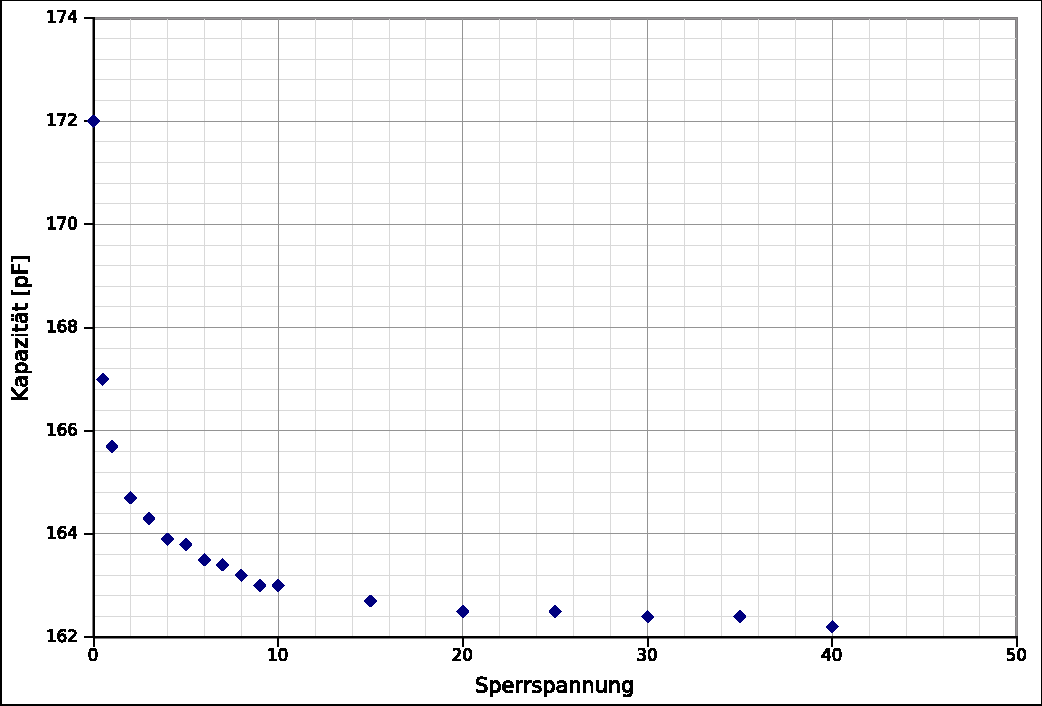
\includegraphics[width=0.8\columnwidth]{messdata.pdf}
    \caption{Kapazität ans Funktion der Sperrspannung}
  \end{figure}
\end{frame}

\subsection{Fazit}
\begin{frame}
\frametitle{Fazit}
  \begin{itemize}
    \item Gleichrichterdioden können als Kapazitätsdioden eingesetzt werden. 
  \end{itemize}
\end{frame}
